\documentclass[11pt]{article}
\usepackage[utf8]{inputenc}
\usepackage{amsmath, amssymb}
\usepackage{graphicx}
\usepackage{hyperref}
\usepackage{geometry}
\usepackage{cite}
\usepackage{listings}

% Geometry settings
\geometry{a4paper, margin=1in}

% Title and author
\title{Title of Your Research Paper}
\author{Your Name \\
University of Alberta \\
\texttt{your.email@example.com}}
\date{\today}

% Code block settings
\lstset{
  basicstyle=\ttfamily\small,
  breaklines=true,
  frame=single,
  numbers=left,
  numberstyle=\tiny,
  xleftmargin=2em,
  language=Python % Change as needed
}

\begin{document}

\maketitle

\begin{abstract}
The abstract provides a concise summary of the research problem, methodology, and findings. It should not exceed 300 words.
\end{abstract}

\section{Introduction}
Introduce the topic, provide background information, and explain the significance of the research. Define the research question or problem.

$$ H =
\begin{pmatrix}
h_1 & h_2 & h_3 \\
h_4 & h_5 & h_6 \\
h_7 & h_8 & 1 \\
\end{pmatrix}
$$.

$$
X = Hx
$$

\section{Related Work}
Summarize relevant prior work in the field. Discuss how your research builds on or differs from existing studies.

\section{Methodology}
Describe the methods or techniques used to conduct the research. Include any specific algorithms, models, or tools you implemented.

\section{Results}
Present your findings clearly using text, tables, and figures. Reference all figures and tables in the text.

\begin{figure}[h!]
\centering
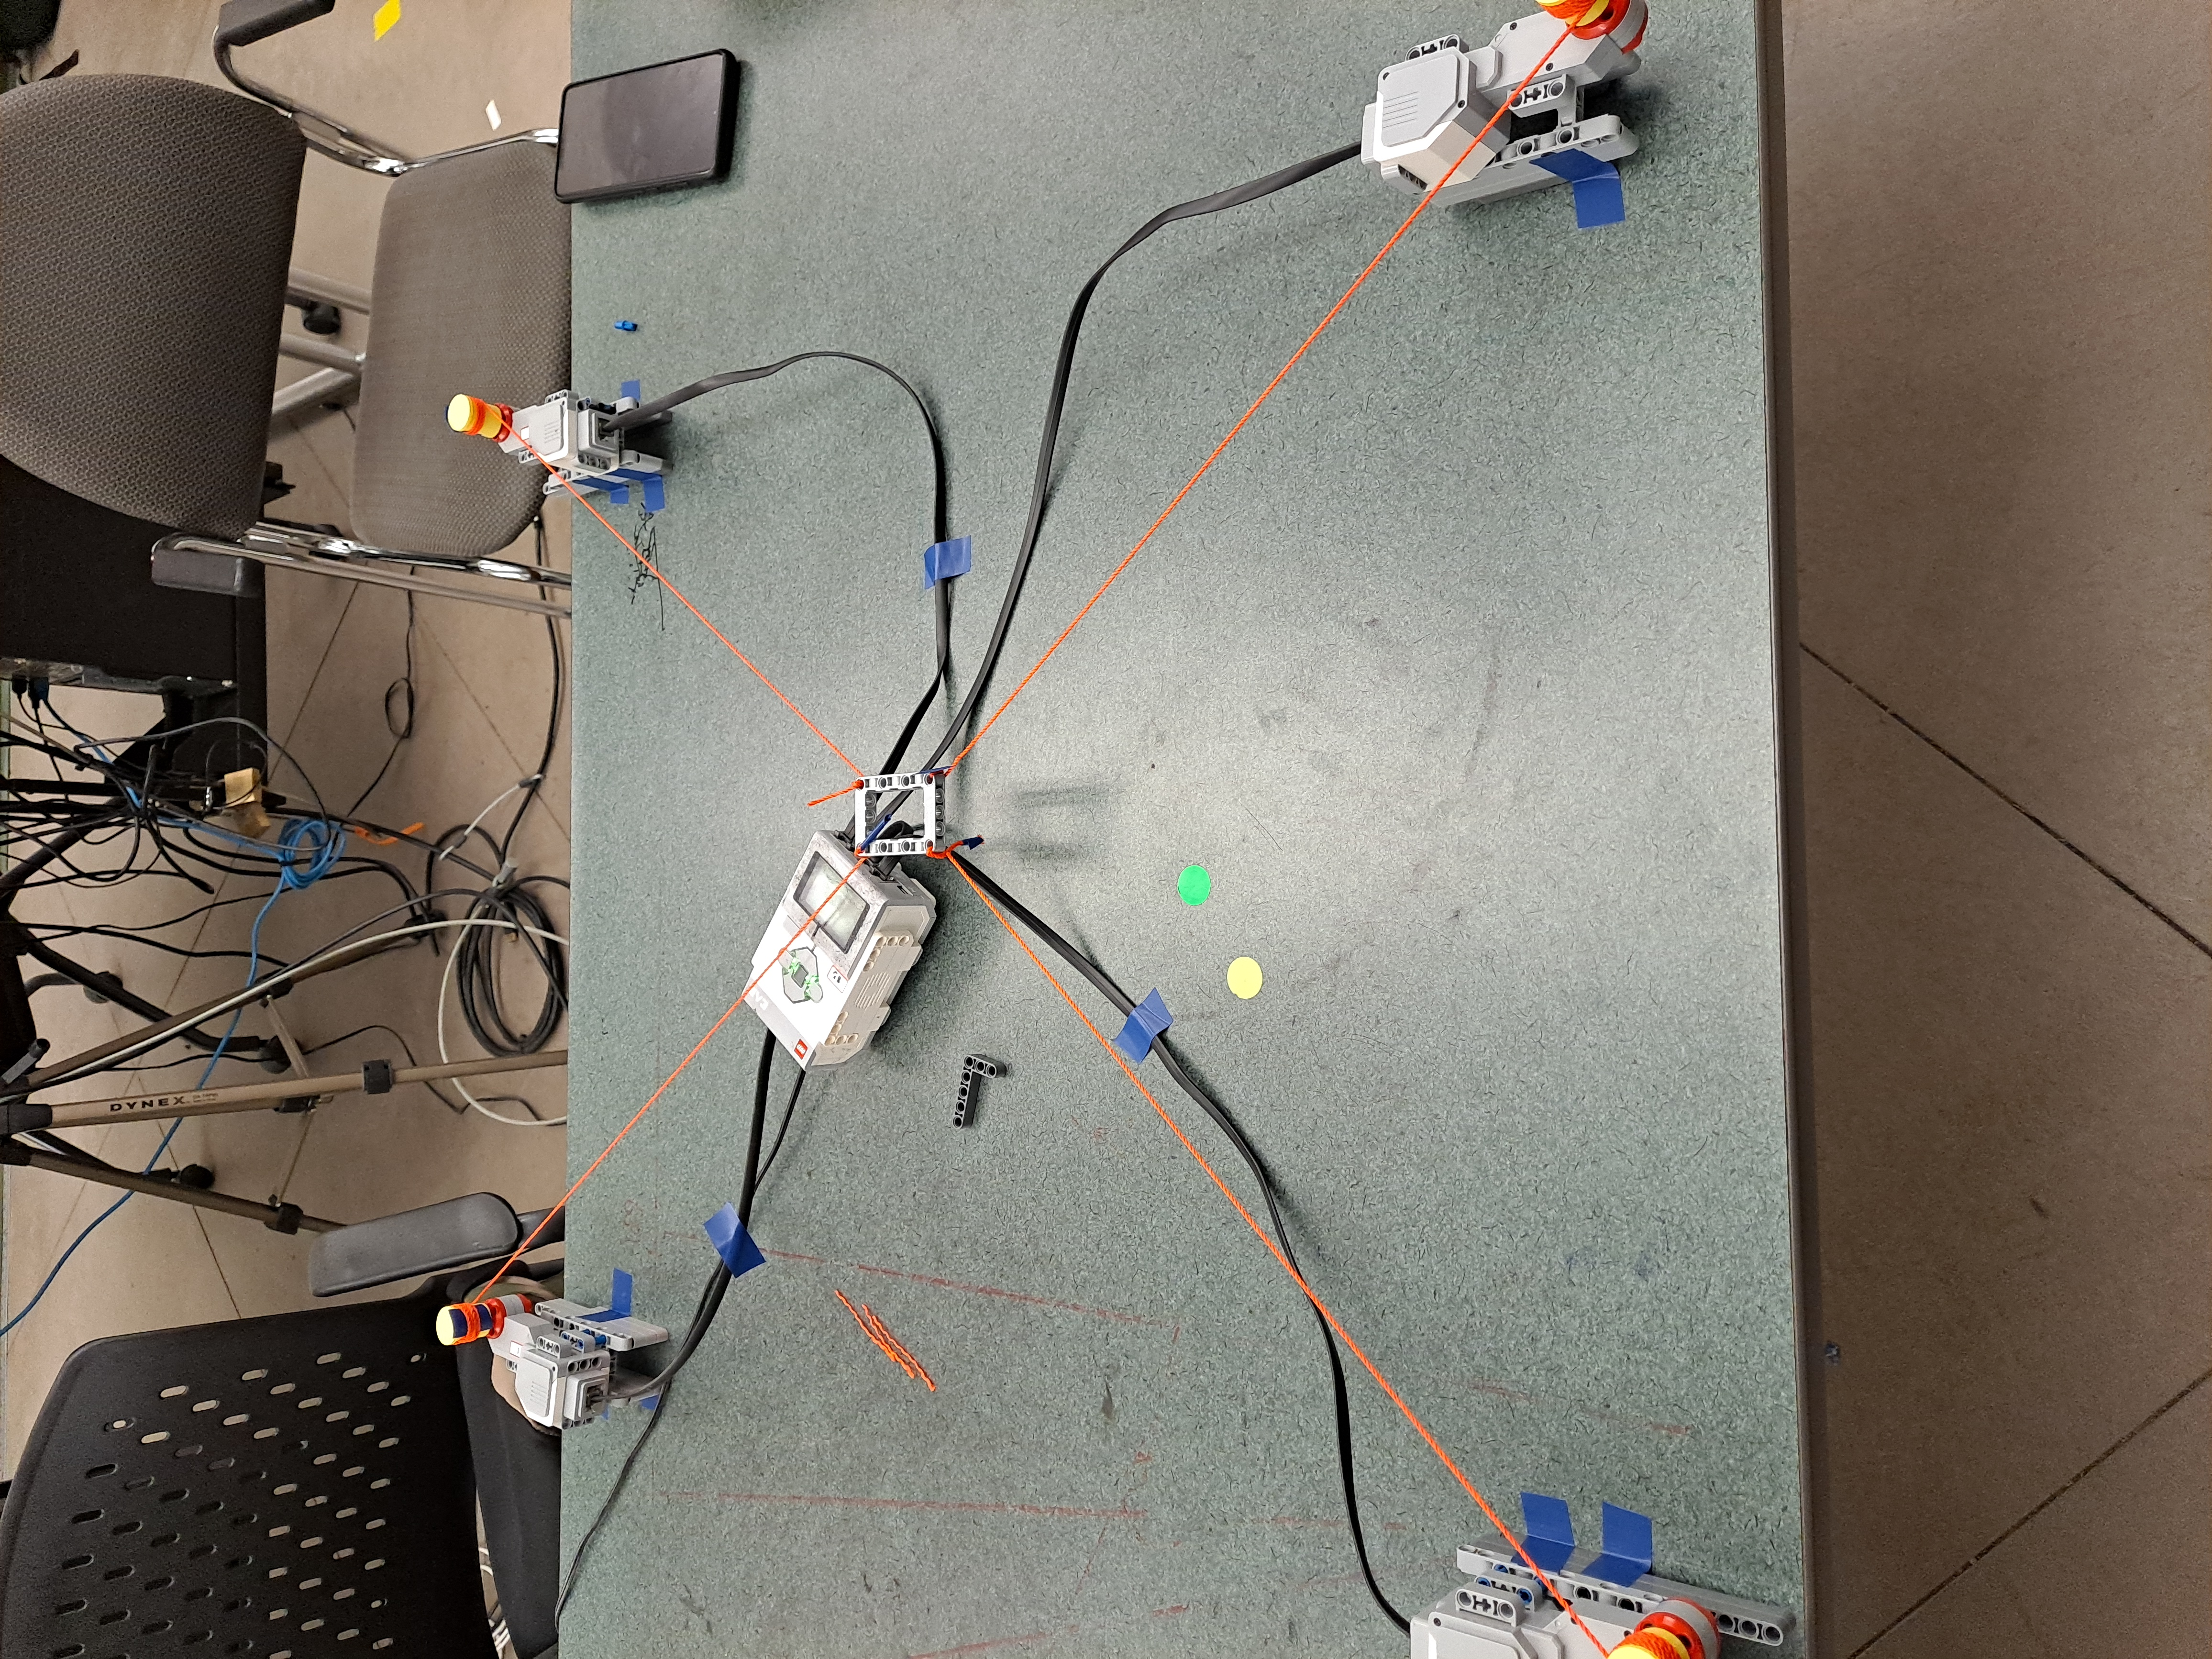
\includegraphics[width=0.5\textwidth]{vision_server/NewTest.jpg} % Replace with your image
\caption{Sample figure caption.}
\label{fig:example}
\end{figure}

\section{Discussion}
Analyze and interpret the results. Discuss their implications, limitations, and potential future work.

\section{Conclusion}
Summarize the key findings and their significance. Suggest directions for further research.

\section*{Acknowledgments}
Optionally acknowledge contributors, funding, or support.

\bibliographystyle{plain}
\bibliography{references}

\appendix
\section{Appendix: Additional Details}
Include supplementary material, code, or data here.

\end{document}
